\documentclass[conference]{IEEEtran}
\IEEEoverridecommandlockouts

\usepackage{iftex}
\ifPDFTeX
  \usepackage[T1]{fontenc}
\else
  \usepackage{fontspec}
  \setmainfont{texgyretermes}[Extension=.otf, UprightFont=*-regular,
    BoldFont=*-bold, ItalicFont=*-italic, BoldItalicFont=*-bolditalic]% Times clone for XeLaTeX/Tectonic
\fi
\usepackage{cite}
\usepackage{amsmath,amssymb,amsfonts}
\usepackage{bm}
\usepackage{graphicx}
\usepackage{booktabs}
\usepackage{tabularx}
\usepackage{array}
\usepackage{xcolor}
\usepackage{tikz}
\usetikzlibrary{arrows.meta,positioning,calc,fit}
\usepackage[hidelinks]{hyperref}
\usepackage{url}

\graphicspath{{figures/}}

% ---------------------------------------------------------------- TikZ styles
\definecolor{boxblue}{HTML}{DCE9F7}
\definecolor{boxgreen}{HTML}{DDF1E1}
\definecolor{boxyellow}{HTML}{FFF2CC}
\definecolor{boxpurple}{HTML}{E6E0F5}
\definecolor{edge}{HTML}{2B3A4A}
\tikzset{
  blk/.style={draw=edge, rounded corners=2pt, line width=0.4pt,
              font=\scriptsize, align=center, inner sep=2.5pt,
              minimum height=4.2mm},
  inb/.style={blk, fill=boxblue},
  prc/.style={blk, fill=boxgreen},
  gat/.style={blk, fill=boxyellow},
  llm/.style={blk, fill=boxpurple},
  arr/.style={-{Latex[length=1.6mm,width=1.2mm]}, draw=edge, line width=0.45pt},
}

\begin{document}

\title{Risk-Aware Multi-Agent Decision-Making for Competitive Food Delivery Platforms: Integrating MAPPO, Distributional Reinforcement Learning, Adaptive Risk, LLM/RAG Guidance, and Explainable AI}

\author{
\IEEEauthorblockN{Uday Kiran}
\IEEEauthorblockA{\textit{Department of Artificial Intelligence}\\
\textit{SVNIT Surat}, India\\
i24ai003@aid.svnit.ac.in}
\and
\IEEEauthorblockN{Santhosh}
\IEEEauthorblockA{\textit{Department of Artificial Intelligence}\\
\textit{SVNIT Surat}, India\\
i24ai006@aid.svnit.ac.in}
\and
\IEEEauthorblockN{Rathan}
\IEEEauthorblockA{\textit{Department of Artificial Intelligence}\\
\textit{SVNIT Surat}, India\\
u24ai025@aid.svnit.ac.in}
\and
\IEEEauthorblockN{Samhitha}
\IEEEauthorblockA{\textit{Department of Artificial Intelligence}\\
\textit{SVNIT Surat}, India\\
u24ai080@aid.svnit.ac.in}
\and
\IEEEauthorblockN{Dr.~Nitesh Funde}
\IEEEauthorblockA{\textit{Department of Artificial Intelligence}\\
\textit{SVNIT Surat}, India\\
nitesh.funde@aid.svnit.ac.in}
}

\maketitle

% ================================================================= ABSTRACT
\begin{abstract}
Two food delivery platforms competing for the same customers must set prices and courier incentives under uncertain demand, limited courier capacity and the moves of a rival. We study this problem with a two-agent simulator and build the decision system in five stages: a market simulator, a Multi-Agent Proximal Policy Optimization (MAPPO) baseline, a distributional critic with a Conditional Value-at-Risk (CVaR) constraint, an adaptive risk estimator combined with retrieval-augmented guidance from FLAN-T5-Small, and an explainability layer that audits the final policy. The language model only contributes a gated action prior; MAPPO still picks the action. Against an adaptive-risk-only control, the full system raised profit per hour by 3.22\% and 4.46\%, raised fulfilment by 2.71 and 3.00 percentage points, and cut tail CVaR by 11.75\% and 9.53\% under normal and shocked demand respectively. Over 8,064 logged decisions, perturbing the features ranked most important flipped 7.4--8.9 times as many actions as perturbing the lowest-ranked ones, which suggests the feature ranking tracks what the policy actually uses.
\end{abstract}

\begin{IEEEkeywords}
Multi-agent reinforcement learning, MAPPO, food delivery, distributional RL, CVaR, retrieval-augmented generation, explainable AI.
\end{IEEEkeywords}

% ================================================================= 1
\section{Introduction}
Online food delivery platforms compete for customers in overlapping cities and time windows, and their main levers (price, promotional incentives and courier allocation) interact. A price cut pulls demand away from a rival, but if the platform has too few couriers on shift that extra demand turns into long waits and cancellations. A platform therefore has to trade profit against fulfilment, delay and service-level targets while reacting to a competitor whose policy it cannot see.

Optimizing expected profit is not enough here. Two pricing policies with the same average return can differ sharply in how badly they do on a bad evening, such as a demand surge during rain with half the fleet offline, and those are the evenings that drive customer churn. We also wanted to know whether a small language model, given retrieved context about the market, could usefully nudge a learned policy without being handed control of it. Finally, a policy that sets prices needs to be inspectable: an operator should be able to ask which inputs drove a decision and check that the answer is faithful to the policy rather than plausible-sounding.

We address these questions with a system built in five stages, each adding one capability to the last (Section~\ref{sec:models}). The contributions are: (i) a two-platform delivery-market simulator calibrated against public order and restaurant data; (ii) a MAPPO policy extended with a 25-quantile distributional critic and a primal-dual CVaR constraint; (iii) an uncertainty-gated way of injecting a language-model action prior into the actor logits, paired with an adaptive risk coefficient; and (iv) an explainability study of the frozen policy that measures feature sensitivity, language-model influence, counterfactuals and the faithfulness of the feature ranking.

% ================================================================= 2
\section{Related Work}
\emph{Multi-agent RL in mobility markets.} Centralized-critic methods such as MADDPG~\cite{lowe2017maddpg} showed that agents in mixed cooperative--competitive settings can be trained with shared information and executed independently. MAPPO applies the clipped surrogate objective of PPO~\cite{schulman2017ppo}, usually with generalized advantage estimation~\cite{schulman2016gae}, in the same way and is a strong baseline in cooperative tasks~\cite{yu2022mappo}. Closest to our domain, multi-agent RL has been used for large-scale fleet management~\cite{lin2018fleet} and ride-hailing order dispatch~\cite{li2019meanfield}. Those works coordinate vehicles within one platform; we instead model two platforms competing on price and incentives.

\emph{Risk-sensitive RL.} Distributional RL models the whole return distribution rather than its mean~\cite{bellemare2017distributional}, learned in practice with quantile regression~\cite{dabney2018qr} or implicit quantile networks~\cite{dabney2018iqn}. CVaR~\cite{rockafellar2000cvar} is the standard tail-risk measure here. It can be optimized by sampling~\cite{tamar2015cvar} or imposed as a constraint in MDPs~\cite{chow2014cvar}, and Lagrangian methods such as RCPO~\cite{tessler2019rcpo} handle general constraints the same way. Garc\'ia and Fern\'andez survey this wider area of safe RL~\cite{garcia2015safe}. Our Model~3 joins the quantile and constrained-CVaR lines.

\emph{Language models as decision aids.} Retrieval-augmented generation~\cite{lewis2020rag} and instruction-tuned text-to-text models such as T5 and FLAN-T5~\cite{raffel2020t5,chung2024flan} are normally used to generate text. In our system the model only scores candidate actions.

\emph{Explainability.} Local surrogate methods (LIME~\cite{ribeiro2016lime}), Shapley-value attributions (SHAP~\cite{lundberg2017shap}) and integrated gradients~\cite{sundararajan2017ig} assign importance to inputs, and counterfactual explanations~\cite{wachter2018counterfactual} describe the smallest input change that alters a decision. Hooker \emph{et al.}~\cite{hooker2019roar} argued that importance rankings must be checked by perturbing the inputs they rank. We follow that idea: a ranking is only useful if perturbing the top-ranked inputs moves the policy more than perturbing the bottom-ranked ones.

% ================================================================= 3
\section{Data and Simulation Environment}

\subsection{Reference Datasets}
Two public datasets were used to calibrate the simulator; the agents never trained on them directly. The Delivery Center dataset~\cite{deliverycenter}, containing food and goods orders from Brazil, gave us hourly demand patterns, delivery-cycle times, hub-level activity and delivery costs. The Zomato Bangalore dataset~\cite{zomato} supplied approximate restaurant price levels, popularity and online-ordering behaviour. All training and evaluation trajectories come from the simulator.

\subsection{Competitive Market Simulator}
The simulator hosts two platforms, Agent~A and Agent~B. At each step both observe their own market state and choose a price and incentive level; the simulator then resolves the joint decision:
\begin{equation}
  s_{t+1} = \mathcal{T}\left(s_t, a_t^{A}, a_t^{B}, \xi_t\right),
\end{equation}
where $s_t$ is the market state, $a_t^{A}$ and $a_t^{B}$ are the two agents' actions, and $\xi_t$ collects the stochastic effects. Demand is time-dependent and stochastic and rises or falls with weather. Customers switch between platforms in response to relative prices and incentives, and orders that exceed available courier capacity either wait or are cancelled. Each step logs revenue, operating and incentive costs, profit, fulfilled and unfulfilled orders, cancellations, delays and SLA outcomes (Fig.~\ref{fig:m1arch}). Evaluation episodes last 168 steps.

\begin{figure}[!t]
\centering
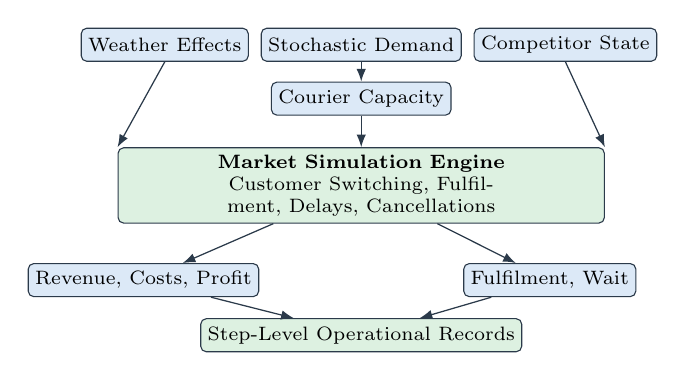
\begin{tikzpicture}[node distance=3mm and 1.5mm]
  \node[inb] (dem) {Stochastic Demand};
  \node[inb, left=of dem] (wea) {Weather Effects};
  \node[inb, right=of dem] (cmp) {Competitor State};
  \node[inb, below=2.5mm of dem] (cap) {Courier Capacity};
  \node[prc, below=4mm of cap, text width=60mm] (eng)
       {\textbf{Market Simulation Engine}\\ Customer Switching, Fulfilment, Delays, Cancellations};
  \node[inb, below left=5mm and -18mm of eng] (rev) {Revenue, Costs, Profit};
  \node[inb, below right=5mm and -18mm of eng] (ful) {Fulfilment, Wait};
  \node[prc, below=12mm of eng] (rec) {Step-Level Operational Records};
  \draw[arr] (wea.south) -- (eng.north west);
  \draw[arr] (cmp.south) -- (eng.north east);
  \draw[arr] (dem) -- (cap);
  \draw[arr] (cap) -- (eng);
  \draw[arr] (eng) -- (rev);
  \draw[arr] (eng) -- (ful);
  \draw[arr] (rev) -- (rec);
  \draw[arr] (ful) -- (rec);
\end{tikzpicture}
\caption{Model 1: competitive market simulator.}
\label{fig:m1arch}
\end{figure}

\subsection{Observations and Actions}
Each agent observes the 14 features in Table~\ref{tab:obs}, covering time of day, weather, smoothed demand, both platforms' prices and incentives, capacity and service quality. Actions are pairs $a_t=(p_t,w_t)$ of one of five price levels and one of five incentive levels, giving $|\mathcal{A}|=25$ discrete actions.

\begin{table}[!t]
\centering
\caption{Fourteen-dimensional observation representation.}
\label{tab:obs}
\small
\begin{tabular}{cl}
\toprule
\textbf{Index} & \textbf{Feature} \\
\midrule
0  & Hour sine component \\
1  & Hour cosine component \\
2  & Normalized day index \\
3  & Rain indicator \\
4  & Normalized EWMA demand \\
5  & Normalized own price \\
6  & Normalized own incentive \\
7  & Normalized competitor price \\
8  & Normalized competitor incentive \\
9  & Capacity ratio \\
10 & Fulfilment EWMA \\
11 & Normalized earnings \\
12 & Normalized waiting time \\
13 & Cancellation EWMA \\
\bottomrule
\end{tabular}
\end{table}

% ================================================================= 4
\section{The Five Models}
\label{sec:models}

\subsection{Model 2: Competitive MAPPO}
Model~1 is the simulator itself. Model~2 replaces hand-written pricing rules with two MAPPO learners~\cite{yu2022mappo} (Fig.~\ref{fig:m2arch}). Each platform has its own actor, a $14\rightarrow128\rightarrow128\rightarrow25$ network with tanh activations that outputs logits for a categorical policy, while training uses information from the shared environment. Actors are updated with the PPO clipped objective~\cite{schulman2017ppo},
\begin{equation}
  L^{CLIP}(\theta) = \mathbb{E}_t\!\left[\min\!\left(r_t(\theta)\hat{A}_t,\,
  \mathrm{clip}\!\left(r_t(\theta),1-\epsilon,1+\epsilon\right)\hat{A}_t\right)\right],
\end{equation}
where $r_t(\theta)=\pi_\theta(a_t\mid o_t)/\pi_{\theta_{\mathrm{old}}}(a_t\mid o_t)$, $\hat{A}_t$ is the advantage estimate and $\epsilon$ is the clip range. The resulting checkpoints initialise Model~3.

\begin{figure}[!t]
\centering
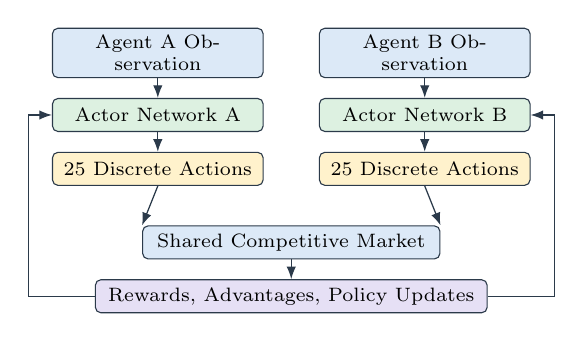
\begin{tikzpicture}[node distance=2.5mm]
  \node[inb, text width=25mm] (oa) {Agent A Observation};
  \node[prc, text width=25mm, below=of oa] (na) {Actor Network A};
  \node[gat, text width=25mm, below=of na] (da) {25 Discrete Actions};
  \node[inb, text width=25mm, right=7mm of oa] (ob) {Agent B Observation};
  \node[prc, text width=25mm, below=of ob] (nb) {Actor Network B};
  \node[gat, text width=25mm, below=of nb] (db) {25 Discrete Actions};
  \path (da.south) -- (db.south) coordinate[midway] (mid);
  \node[inb, text width=36mm, below=5mm of mid] (mk) {Shared Competitive Market};
  \node[llm, text width=48mm, below=of mk] (up) {Rewards, Advantages, Policy Updates};
  \draw[arr] (oa) -- (na); \draw[arr] (na) -- (da);
  \draw[arr] (ob) -- (nb); \draw[arr] (nb) -- (db);
  \draw[arr] (da.south) -- (mk.north west);
  \draw[arr] (db.south) -- (mk.north east);
  \draw[arr] (mk) -- (up);
  \draw[arr] (up.west) -| ([xshift=-3mm]na.west) -- (na.west);
  \draw[arr] (up.east) -| ([xshift=3mm]nb.east) -- (nb.east);
\end{tikzpicture}
\caption{Two-agent MAPPO architecture.}
\label{fig:m2arch}
\end{figure}

\subsection{Model 3: Distributional Critic and CVaR Constraint}
A mean return hides the bad tail. Model~3 therefore swaps the scalar critic for one that predicts $N_q=25$ return quantiles $Z(s)=\{z_1(s),\ldots,z_{25}(s)\}$, trained with the quantile Huber loss~\cite{dabney2018qr},
\begin{equation}
  L_\kappa = \frac{1}{N_q}\sum_{i=1}^{N_q}\left|\tau_i - \mathbb{I}(\delta_i < 0)\right| \mathcal{L}_\kappa(\delta_i),
\end{equation}
with $\delta_i$ the TD error of quantile $i$. From these quantiles we estimate CVaR at $\alpha=0.10$, the mean of the worst 10\% of outcomes, and impose it as a constraint~\cite{chow2014cvar}:
\begin{equation}
  \mathcal{L}(\pi,\lambda) = J(\pi) - \lambda\left(\mathrm{CVaR}_\alpha(\pi) - C\right),
\end{equation}
which is the Lagrangian of $\max_\pi J(\pi)$ subject to $\mathrm{CVaR}_\alpha(\pi)\le C$; $\lambda$ is updated by dual ascent (Fig.~\ref{fig:m3arch}). Compared with Model~2, fulfilment rose from 0.852 to 0.867 and tail CVaR fell from 4.545 to 4.111, a 9.55\% reduction.

\begin{figure}[!t]
\centering
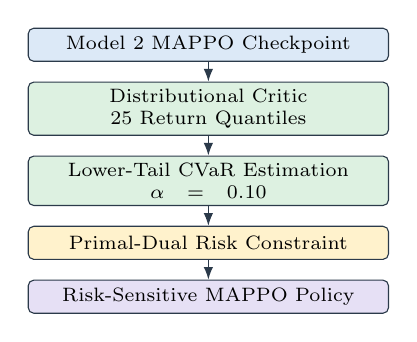
\begin{tikzpicture}[node distance=2.5mm]
  \node[inb, text width=44mm] (c) {Model 2 MAPPO Checkpoint};
  \node[prc, text width=44mm, below=of c] (d) {Distributional Critic\\ 25 Return Quantiles};
  \node[prc, text width=44mm, below=of d] (v) {Lower-Tail CVaR Estimation\\ $\alpha = 0.10$};
  \node[gat, text width=44mm, below=of v] (p) {Primal-Dual Risk Constraint};
  \node[llm, text width=44mm, below=of p] (r) {Risk-Sensitive MAPPO Policy};
  \foreach \a/\b in {c/d,d/v,v/p,p/r} \draw[arr] (\a) -- (\b);
\end{tikzpicture}
\caption{Distributional and CVaR-constrained learning architecture.}
\label{fig:m3arch}
\end{figure}

\subsection{Model 4: Adaptive Risk and Gated LLM/RAG Guidance}
Model~4 adds two things to the risk-sensitive policy (Fig.~\ref{fig:m4arch}). The first is an adaptive risk coefficient. An estimator reads observable market signals and their recent history, without access to any hidden shock label, and outputs a risk score $r_t\in[0,1]$ that sets $\lambda_t = 0.10 + 0.50\,r_t$, so the policy becomes more conservative when conditions look stressed.

The second is guidance from a language model. Retrieved market context~\cite{lewis2020rag} is passed to FLAN-T5-Small~\cite{chung2024flan,flant5small}. Our first attempt asked the model to generate a structured action; we later replaced this with a contrastive scheme: the model scores the likelihood of each of the 25 price--incentive combinations, and these scores are normalised into a prior $P_{\mathrm{LLM}}(a\mid s)$. A confidence gate $g_t$ decides how much of that prior reaches the actor:
\begin{equation}
  \ell_{\mathrm{combined}} = \ell_{\mathrm{RL}} + g_t \log\left(P_{\mathrm{LLM}}(a \mid s) + \varepsilon\right),
\end{equation}
where $\ell_{\mathrm{RL}}$ are the MAPPO logits and $\varepsilon$ is a small constant. Because the prior only shifts logits, MAPPO still chooses the action.

\begin{figure}[!t]
\centering
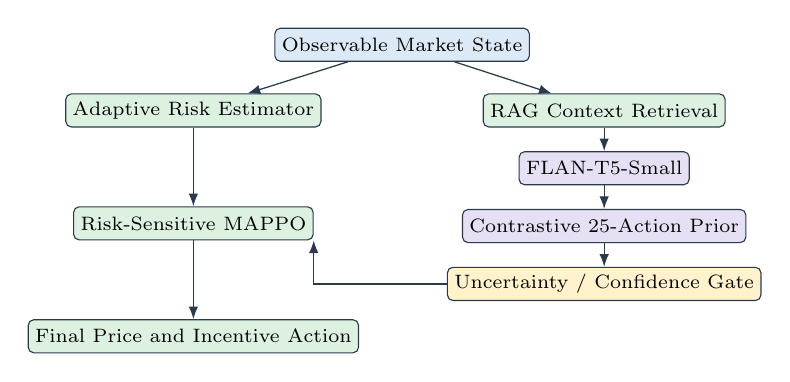
\begin{tikzpicture}[node distance=3mm and 2mm]
  \node[inb] (st) {Observable Market State};
  \node[prc, below left=4mm and -6mm of st] (re) {Adaptive Risk Estimator};
  \node[prc, below right=4mm and -6mm of st] (rg) {RAG Context Retrieval};
  \node[llm, below=of rg] (ft) {FLAN-T5-Small};
  \node[llm, below=of ft] (pr) {Contrastive 25-Action Prior};
  \node[gat, below=of pr] (gt) {Uncertainty / Confidence Gate};
  \node[prc, below=10mm of re] (mp) {Risk-Sensitive MAPPO};
  \node[prc, below=10mm of mp] (fa) {Final Price and Incentive Action};
  \draw[arr] (st) -- (re); \draw[arr] (st) -- (rg);
  \draw[arr] (rg) -- (ft); \draw[arr] (ft) -- (pr); \draw[arr] (pr) -- (gt);
  \draw[arr] (re) -- (mp);
  \draw[arr] (gt.west) -| (mp.south east);
  \draw[arr] (mp) -- (fa);
\end{tikzpicture}
\caption{Model 4: adaptive-risk and uncertainty-gated LLM/RAG integration.}
\label{fig:m4arch}
\end{figure}

The full Model~4 policy was trained for 1,500 updates, making 3,000 calls to the language model with no parse failures; the adaptive-risk-only control, which omits the language-model prior, was trained for 1,000 updates.

\subsection{Model 5: Explaining the Frozen Policy}
Model~5 trains nothing. It freezes the Model~4 policy and asks two questions: which inputs drive its decisions, and does the resulting ranking reflect the policy's real behaviour? Every decision is logged with its observation, action probabilities, chosen action, risk score, language-model prior, gate value and simulator outcome. A pilot of 672 decisions over two episodes checked the pipeline before the full runs, which logged 4,032 decisions in each condition.

\emph{Feature sensitivity} perturbs one input at a time and measures the change in the chosen action's preference, logit margin, action probabilities and stability. \emph{LLM influence} compares the full policy with the same policy with the prior removed, recording the gate value, how often the action changes, KL divergence and logit change. \emph{Counterfactuals} search for realistic single-feature changes that alter the chosen action while the logged prior and gate are held fixed, so only the observation effect is measured. \emph{Faithfulness} perturbs the top-ranked and bottom-ranked features and compares the resulting action-flip rates and margin changes; if the ranking is faithful, both ratios should be well above one.

% ================================================================= 5
\section{Results}

\subsection{Is the Shock Real?}
The shock condition raises the simulator's demand-volatility parameter from $\sigma_\lambda=0.12$ to $0.30$. Before comparing policies, we checked that this change actually reaches the evaluated episodes. Recovering the demand noise from 672 steps per condition gave standard deviations of 0.1193 and 0.2940, a ratio of 2.46 against the configured 2.50; mean absolute noise rose from 0.0960 to 0.2365 and its 95th percentile from 0.2344 to 0.5685 (Fig.~\ref{fig:shock}).

\begin{figure}[!t]
\centering
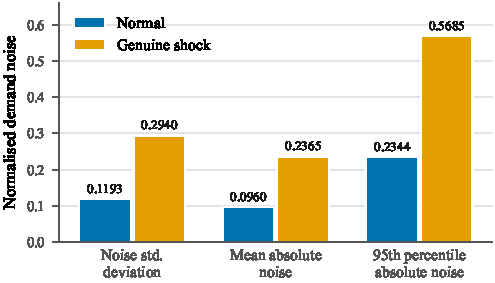
\includegraphics[width=\columnwidth]{fig_shock_validation}
\caption{Shock-condition validation: standard deviation, mean absolute value, and 95th percentile absolute value of the recovered normalised demand noise, computed from 672 simulation steps in each condition.}
\label{fig:shock}
\end{figure}

The risk estimator picked this up without being told. Its mean score was 0.4072 under normal demand and 0.7019 under shock, and its spread roughly doubled (standard deviation 0.0608 versus 0.1208, Fig.~\ref{fig:risk}).

\begin{figure}[!t]
\centering
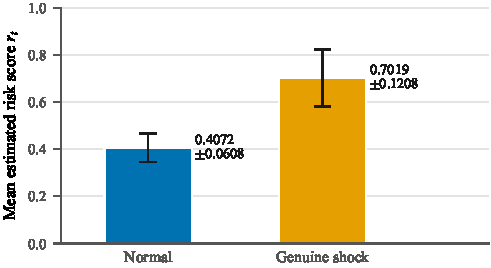
\includegraphics[width=\columnwidth]{fig_risk_estimator}
\caption{Response of the adaptive risk estimator. Bars give the mean estimated risk score $r_t$ over 4,032 decision records per condition; error bars give $\pm 1$ standard deviation of the per-decision score (not a confidence interval).}
\label{fig:risk}
\end{figure}

\subsection{Model 4 Against the Adaptive-Risk Control}
Table~\ref{tab:m4} and Fig.~\ref{fig:m4perf} compare the full system with its control. Adding the gated prior improved all three metrics in both conditions. The profit gain was larger under shock (4.46\% versus 3.22\%), as was the fulfilment gain (3.00 versus 2.71 points), while the CVaR reduction was somewhat smaller (9.53\% versus 11.75\%).

\begin{table}[!t]
\centering
\caption{Adaptive-risk control (Ctrl) versus full Model 4.}
\label{tab:m4}
\small
\setlength{\tabcolsep}{3pt}
\begin{tabular}{lccr}
\toprule
\textbf{Metric} & \textbf{Ctrl} & \textbf{Model 4} & \textbf{Change} \\
\midrule
\multicolumn{4}{l}{\emph{Normal market}} \\
Profit per hour & 344.90 & 356.00 & +3.22\% \\
Fulfilment rate & 0.8504 & 0.8775 & +2.71 pp \\
Tail CVaR       & 4.8128 & 4.2483 & $-$11.75\% \\
\midrule
\multicolumn{4}{l}{\emph{Genuine shock}} \\
Profit per hour & 314.24 & 328.26 & +4.46\% \\
Fulfilment rate & 0.8124 & 0.8424 & +3.00 pp \\
Tail CVaR       & 5.3776 & 4.8655 & $-$9.53\% \\
\bottomrule
\end{tabular}
\end{table}

\begin{figure*}[!t]
\centering
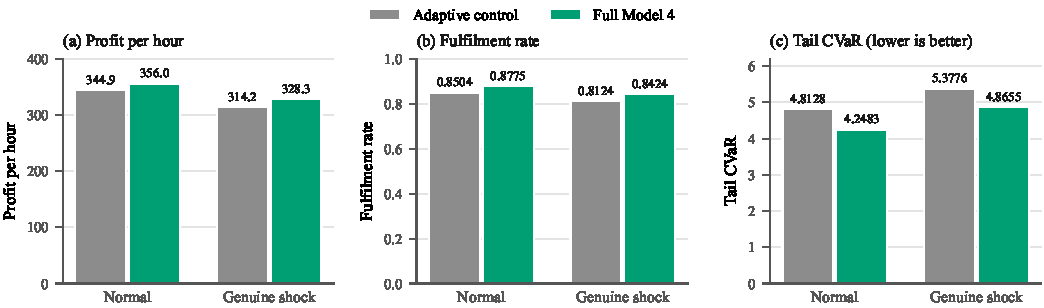
\includegraphics[width=\textwidth]{fig_model4_performance}
\caption{Model 4 performance comparison between the adaptive-risk-only control and the full Model 4 system under normal and genuine-shock conditions: (a) profit per hour, (b) fulfilment rate, and (c) tail CVaR, where a lower value indicates a smaller downside risk. Values are taken from Table~\ref{tab:m4}.}
\label{fig:m4perf}
\end{figure*}

\subsection{What Drives the Policy}
The seven most influential features, in order, were the two hour-of-day components, smoothed demand, waiting time, competitor price, own price and capacity ratio. Time of day dominating the ranking is unsurprising given how strongly demand follows the daily cycle in the simulator.

The language model's influence is small. The mean gate value was about 0.13 in both conditions, and removing the prior changed the chosen action in only 1.54\% of normal and 1.84\% of shock decisions (Table~\ref{tab:xai}). The mean KL divergence between the full and RL-only policies was $1.906\times10^{-4}$ and $1.785\times10^{-4}$, with a mean absolute logit change near 0.5 (Fig.~\ref{fig:llmcf}a). The prior seems to act as a tie-breaker on close decisions rather than as a second controller, yet the profit and CVaR gains in Table~\ref{tab:m4} show that these rare interventions still matter.

The counterfactual search found 363 and 364 successful counterfactuals, covering about 36\% of sampled decisions, with a feature-level flip rate near 10\% (Fig.~\ref{fig:llmcf}b).

\begin{table}[!t]
\centering
\caption{Model 5 explainability results.}
\label{tab:xai}
\small
\setlength{\tabcolsep}{4pt}
\begin{tabular}{lcc}
\toprule
\textbf{Measurement} & \textbf{Normal} & \textbf{Genuine Shock} \\
\midrule
Decision records                 & 4,032          & 4,032 \\
Mean adaptive risk               & 0.4072         & 0.7019 \\
Mean LLM gate                    & 0.1340         & 0.1322 \\
LLM action-change rate           & 1.54\%         & 1.84\% \\
Top/bottom action-flip ratio     & 7.38$\times$   & 8.86$\times$ \\
Top/bottom margin ratio          & 20.33$\times$  & 21.21$\times$ \\
Counterfactual decision coverage & 36.33\%        & 35.94\% \\
\bottomrule
\end{tabular}
\end{table}

\begin{figure*}[!t]
\centering
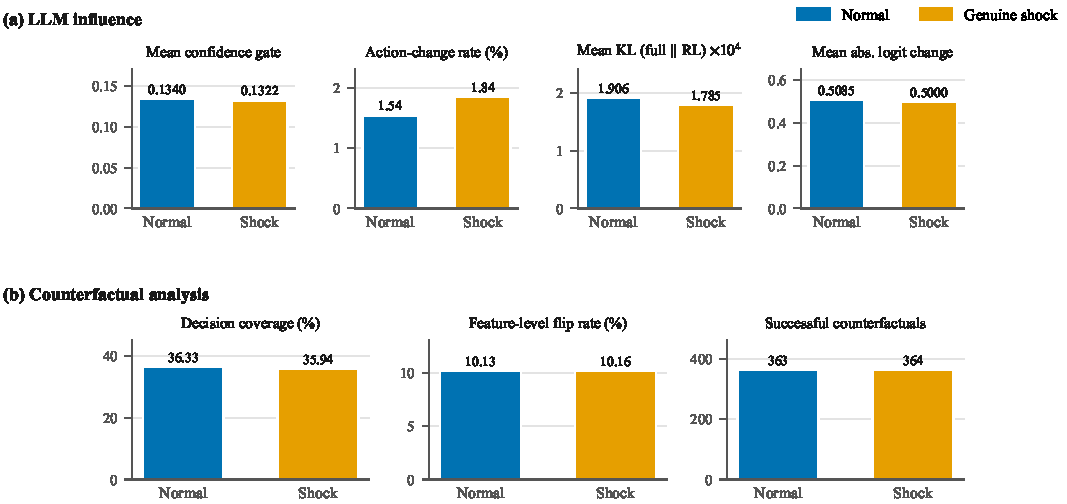
\includegraphics[width=\textwidth]{fig_llm_counterfactual}
\caption{LLM influence and counterfactual analysis under normal and genuine-shock conditions. (a) LLM influence: mean confidence gate, action-change rate, mean KL divergence between the full and RL-only policies, and mean absolute logit change. (b) Counterfactual analysis: unique decision coverage, feature-level flip rate, and number of successful counterfactuals. Each panel uses its own axis because the metrics differ in scale and unit.}
\label{fig:llmcf}
\end{figure*}

\subsection{Is the Ranking Faithful?}
With 256 perturbed samples per group, perturbing the top-ranked features flipped 23.0\% of actions under normal demand, against 3.1\% for the bottom-ranked features; under shock the rates were 24.2\% and 2.7\% (Fig.~\ref{fig:faith}). Mean absolute margin change was 1.407 versus 0.069 and 1.455 versus 0.069. This gives flip ratios of 7.38 and 8.86 and margin ratios of 20.33 and 21.21, so the features we call important are the ones the policy actually responds to.

\begin{figure}[!t]
\centering
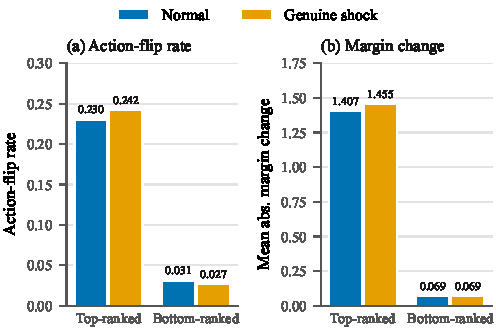
\includegraphics[width=\columnwidth]{fig_faithfulness}
\caption{Explanation faithfulness: (a) action-flip rate and (b) mean absolute action-margin change when the top-ranked and bottom-ranked features are perturbed, under normal and genuine-shock conditions (256 samples per group).}
\label{fig:faith}
\end{figure}

% ================================================================= 6
\section{Discussion and Conclusion}
Fig.~\ref{fig:full} shows how the pieces fit together. Each stage was tested against the one before: the CVaR constraint lowered tail risk relative to plain MAPPO, and the gated language-model prior improved profit, fulfilment and tail risk relative to adaptive risk alone, in both normal and shocked markets. The explainability layer then showed that the policy relies mainly on time of day, demand, waiting time and the two prices, and that this ranking holds up under a faithfulness test.

\begin{figure}[!t]
\centering
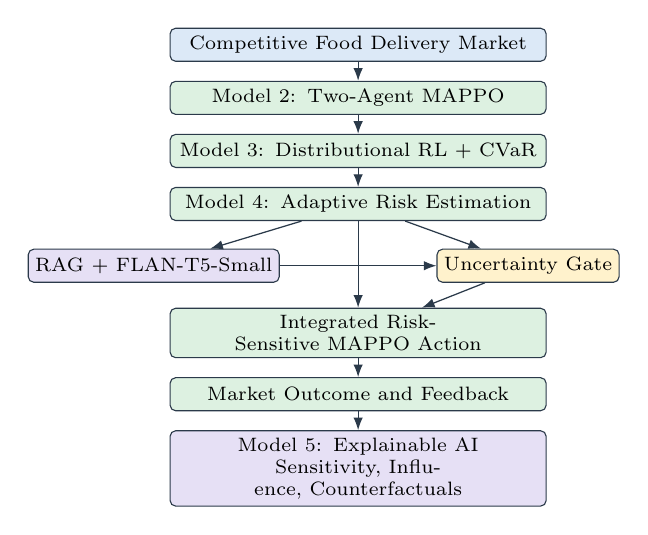
\begin{tikzpicture}[node distance=2.4mm and 2mm]
  \node[inb, text width=46mm] (mk) {Competitive Food Delivery Market};
  \node[prc, text width=46mm, below=of mk] (m2) {Model 2: Two-Agent MAPPO};
  \node[prc, text width=46mm, below=of m2] (m3) {Model 3: Distributional RL + CVaR};
  \node[prc, text width=46mm, below=of m3] (m4) {Model 4: Adaptive Risk Estimation};
  \node[llm, below left=3.5mm and -14mm of m4] (rg) {RAG + FLAN-T5-Small};
  \node[gat, below right=3.5mm and -14mm of m4] (ug) {Uncertainty Gate};
  \node[prc, text width=46mm, below=11mm of m4] (ac) {Integrated Risk-Sensitive MAPPO Action};
  \node[prc, text width=46mm, below=of ac] (fb) {Market Outcome and Feedback};
  \node[llm, text width=46mm, below=of fb] (m5) {Model 5: Explainable AI\\ Sensitivity, Influence, Counterfactuals};
  \foreach \a/\b in {mk/m2,m2/m3,m3/m4,m4/ac,ac/fb} \draw[arr] (\a) -- (\b);
  \draw[arr] (m4) -- (rg); \draw[arr] (m4) -- (ug);
  \draw[arr] (rg) -- (ug);
  \draw[arr] (ug) -- (ac);
  \draw[arr, dashed] (fb) -- (m5);
\end{tikzpicture}
\caption{Complete system. Model 5 analyses the frozen integrated policy.}
\label{fig:full}
\end{figure}

Several limits apply. All results come from a simulator, calibrated to public data but not validated against live platform outcomes. The full system and its control were trained for different numbers of updates (1,500 and 1,000), so part of the gain may come from extra training rather than from the prior. The Model~4 comparison is reported without confidence intervals across training seeds. Finally, the language model is very small; whether a larger model would earn a higher gate value, or simply add cost, is an open question. Matching training budgets and reporting variation across seeds are the natural next steps.

% ================================================================= REFERENCES
\begin{thebibliography}{25}

\bibitem{schulman2017ppo}
J.~Schulman, F.~Wolski, P.~Dhariwal, A.~Radford, and O.~Klimov, ``Proximal policy optimization algorithms,'' \emph{arXiv preprint arXiv:1707.06347}, 2017.

\bibitem{yu2022mappo}
C.~Yu \emph{et al.}, ``The surprising effectiveness of PPO in cooperative multi-agent games,'' in \emph{Advances in Neural Information Processing Systems}, 2022.

\bibitem{bellemare2017distributional}
M.~G. Bellemare, W.~Dabney, and R.~Munos, ``A distributional perspective on reinforcement learning,'' in \emph{Proc. Int. Conf. Machine Learning}, 2017.

\bibitem{dabney2018qr}
W.~Dabney, M.~Rowland, M.~G. Bellemare, and R.~Munos, ``Distributional reinforcement learning with quantile regression,'' in \emph{Proc. AAAI Conf. Artificial Intelligence}, 2018.

\bibitem{rockafellar2000cvar}
R.~T. Rockafellar and S.~Uryasev, ``Optimization of conditional value-at-risk,'' \emph{Journal of Risk}, vol.~2, pp.~21--41, 2000.

\bibitem{chow2014cvar}
Y.~Chow and M.~Ghavamzadeh, ``Algorithms for CVaR optimization in MDPs,'' in \emph{Advances in Neural Information Processing Systems}, vol.~27, 2014.

\bibitem{lewis2020rag}
P.~Lewis \emph{et al.}, ``Retrieval-augmented generation for knowledge-intensive NLP tasks,'' in \emph{Advances in Neural Information Processing Systems}, 2020.

\bibitem{chung2024flan}
H.~W. Chung \emph{et al.}, ``Scaling instruction-finetuned language models,'' \emph{Journal of Machine Learning Research}, vol.~25, 2024.

\bibitem{sundararajan2017ig}
M.~Sundararajan, A.~Taly, and Q.~Yan, ``Axiomatic attribution for deep networks,'' in \emph{Proc. Int. Conf. Machine Learning}, 2017.

\bibitem{deliverycenter}
Delivery Center, ``Food and goods orders in Brazil,'' Kaggle dataset. [Online]. Available: \url{https://www.kaggle.com/datasets/nosbielcs/brazilian-delivery-center}

\bibitem{zomato}
H.~P. Himanshu, ``Zomato Bangalore restaurants,'' Kaggle dataset. [Online]. Available: \url{https://www.kaggle.com/datasets/himanshupoddar/zomato-bangalore-restaurants}

\bibitem{flant5small}
Google Research, ``FLAN-T5-Small,'' Hugging Face Model Repository. [Online]. Available: \url{https://huggingface.co/google/flan-t5-small}

\bibitem{lowe2017maddpg}
R.~Lowe, Y.~Wu, A.~Tamar, J.~Harb, P.~Abbeel, and I.~Mordatch, ``Multi-agent actor-critic for mixed cooperative-competitive environments,'' in \emph{Advances in Neural Information Processing Systems}, vol.~30, 2017.

\bibitem{schulman2016gae}
J.~Schulman, P.~Moritz, S.~Levine, M.~Jordan, and P.~Abbeel, ``High-dimensional continuous control using generalized advantage estimation,'' in \emph{Proc. Int. Conf. Learning Representations}, 2016.

\bibitem{lin2018fleet}
K.~Lin, R.~Zhao, Z.~Xu, and J.~Zhou, ``Efficient large-scale fleet management via multi-agent deep reinforcement learning,'' in \emph{Proc. ACM SIGKDD Int. Conf. Knowledge Discovery \& Data Mining}, 2018, pp.~1774--1783.

\bibitem{li2019meanfield}
M.~Li, Z.~Qin, Y.~Jiao, Y.~Yang, J.~Wang, C.~Wang, G.~Wu, and J.~Ye, ``Efficient ridesharing order dispatching with mean field multi-agent reinforcement learning,'' in \emph{Proc. World Wide Web Conf.}, 2019, pp.~983--994.

\bibitem{dabney2018iqn}
W.~Dabney, G.~Ostrovski, D.~Silver, and R.~Munos, ``Implicit quantile networks for distributional reinforcement learning,'' in \emph{Proc. Int. Conf. Machine Learning}, 2018, pp.~1096--1105.

\bibitem{tamar2015cvar}
A.~Tamar, Y.~Glassner, and S.~Mannor, ``Optimizing the CVaR via sampling,'' in \emph{Proc. AAAI Conf. Artificial Intelligence}, 2015.

\bibitem{tessler2019rcpo}
C.~Tessler, D.~J. Mankowitz, and S.~Mannor, ``Reward constrained policy optimization,'' in \emph{Proc. Int. Conf. Learning Representations}, 2019.

\bibitem{garcia2015safe}
J.~Garc\'ia and F.~Fern\'andez, ``A comprehensive survey on safe reinforcement learning,'' \emph{Journal of Machine Learning Research}, vol.~16, no.~1, pp.~1437--1480, 2015.

\bibitem{raffel2020t5}
C.~Raffel \emph{et al.}, ``Exploring the limits of transfer learning with a unified text-to-text transformer,'' \emph{Journal of Machine Learning Research}, vol.~21, no.~140, pp.~1--67, 2020.

\bibitem{ribeiro2016lime}
M.~T. Ribeiro, S.~Singh, and C.~Guestrin, ``\,`Why should I trust you?': Explaining the predictions of any classifier,'' in \emph{Proc. ACM SIGKDD Int. Conf. Knowledge Discovery \& Data Mining}, 2016, pp.~1135--1144.

\bibitem{lundberg2017shap}
S.~M. Lundberg and S.-I. Lee, ``A unified approach to interpreting model predictions,'' in \emph{Advances in Neural Information Processing Systems}, vol.~30, 2017.

\bibitem{wachter2018counterfactual}
S.~Wachter, B.~Mittelstadt, and C.~Russell, ``Counterfactual explanations without opening the black box: Automated decisions and the GDPR,'' \emph{Harvard Journal of Law \& Technology}, vol.~31, no.~2, pp.~841--887, 2018.

\bibitem{hooker2019roar}
S.~Hooker, D.~Erhan, P.-J. Kindermans, and B.~Kim, ``A benchmark for interpretability methods in deep neural networks,'' in \emph{Advances in Neural Information Processing Systems}, vol.~32, 2019.

\end{thebibliography}

\end{document}
